%Réalisation technique
    %Contexte technique opérationnel
        %Plan de vol et reports ADSC
        %Plate-forme TIARE (production de log fichiers texte)
    %Base de travail
        %Python : librairies, IDE, Linux
        %Google Earth
    %Conception Produit
            %Le programme réalisé et ses fonctions
                %Analyse DATASET
                %Analyse du trafic
    %Problèmes techniques rencontrés
            %Rotondité, intersection, zip, optimisation dans google earth….



Avant de passer à la pratique un apprentissage théorique à du etre réalisé.

\section{Le contexte technique operationel}

    \subsection{\textsc{EurocatX}}
Il faut bien comprendre comment marche le système afin de bien visulaliser d'où proviennent les informations. Comme décrit grossièrement dans le schéma (cf. Fig. \vref{eurocatx}),
\begin{figure}
    \center
    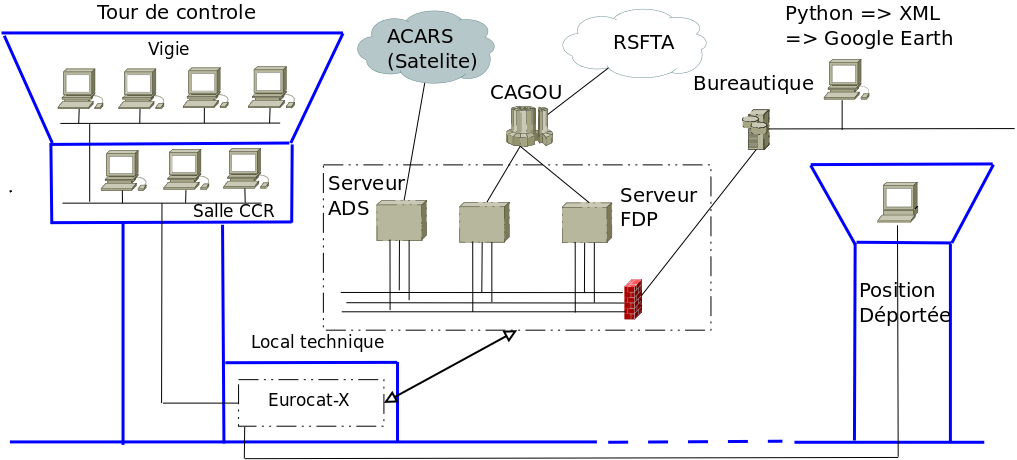
\includegraphics[width=15cm]{images/SchemaControle.png}
    \caption{Schématisation du système \textsc{EurocatX} au niveau des tour de controle}
    \label{eurocatx}
\end{figure}
\textsc{EurocatX} récupere les information sur les plans de vol par l'intermediaire de \textsc{Cagou}\footnote{\textsc{Cagou}: nom donné au commutateur \textsc{Rsfta}}. Il rcupère aussi le positionement émis par l'avion à l'aide de la transmition Satelite, \textsc{Vhf}\footnote{\textsc{Vhf}: Very High Frequency, soit une bande radio de très haute frequance} ou des données radars lors de son approche. Le système \textsc{EurocatX} donne un acces à la bureautique protégé par un parfeu (FireWall) afin de rendre disponible sur ce réseau un certain nombre d'information. Dans notre cas nous y recupererons:
\begin{itemize}
    \item toutes les données de configuration du système tels que les nom et coordonnées des balise referancée, la position des zone de controle et des zone \textsc{Aci} ou encore les route utilisée pour décrire les plans de vols.
    \item Les fichiers de log du Commutateur \textsc{Cagou} afin de pouvoir exploiter les plans de vol reçus par le réseaux \textsc{Rsfta}.
    \item Tous les report \textsc{Ads} reçu par satelite et traité par le systeme.
\end{itemize} 
Le système envoye les information recoltées et celle calculées au visues\footnote{Visue: Nom pour décrire les ordinateur utilisés pour visualiser les données de controles} situées dans la tour de controle au niveau de la Vigie ou de la salle \textsc{Ccr} ainsi que de la position deportée à \textsc{Morea}.

Les données seront donc recupérée dans les fichiers ".asf" pour tous ce qui est de la configuration du système, dans les fichier du \textsc{Fdp} pour les plans de vol et dans les fichiers du serveur \textsc{Ads} pour les repport ainsi que pour la position calculée des aéronefs.

    \subsection{Le domaine de l'aviation}
Il m'a aussi été nécessaire de prendre connaissance de touts les terme, unité, convention et j'en passe utilisé dans le domaine aéronautique.

        \subsubsection{Les coordonnées et unités:}
Tout d'abord est vite venu le problème de conversion de coordonnées, J'ai donc du revoir les conversions de coordonnées sphériques ainsi que les conversions de distances.
J'ai également du, comme expliquée ci dessus (cf. \vref{mathcoord})
me remémoré les manière de calculé le point d'intersection de deux arc de cercle en coordonnées sphériques.

        \subsubsection{Convention:}
Plusieurs conventions on du être acquise comme celle utilisé par le système TIARE pour décrire les report \textsc{Ads} ou encre celle utilisée par les compagnie pour le dépôt de plan de vole.
NE PAS OUBLIER DE FAIR REF AU DOCUMLENT 4444 ...





\section{Base de travail}
    \subsection{Le langage Python}
        \subsubsection{Bien coder:\label{pygood}}
Afin de pouvoir apprendre les bonne pratique de la programmation Python\cite{pybook} j'ai lu (en diagonale) un livre tres bien expliqué intitulé Programation Python, conception et Optimisation. Celui-ci m'a permit de pouvoir d'une part revoir ce qui avait été appliquer lors de mes etudes et d'autre part avoir une vue global sur le langage et ainsi pouvoir prendre du recule lors du codage.

Celui ci m'a par exemple appris le nouveau style de programmation qui part du principe que chaque nouvel objet définit est basé sur un Objet existant, et que par la même occasion tout en python était Objet (même une simple variable booléene). Ou encore la maniere de verifier si un objet etait faux, egale à 0 ou encore une chaine vide simplement en demandant si il existait (ex:~\texttt{"if x != 0:"}~devient \texttt{"if not x:"})

        \subsubsection{Utiliser les expression régulière:} 
L'apprentissage de l'utilisation des expression réguliere\footnote{Une expression régulière
 est en informatique une chaîne de caractères que l’on appelle parfois un motif et qui décrit un ensemble de chaînes de caractères possibles selon une syntaxe précise.}, m'a été grandement facilité garce au site: \url{http://www.dsimb.inserm.fr/}\cite{re} et a la documentation en ligne de Python\cite{pydoc}. Il s'est avéré après apprentissage que ces expression régulière auron grandement facilité la faisabilité du projet.

        \subsubsection{L'optimisation:}
Je pourrais cité un passage du livre qui dit:
\begin{quotation}
    Fourni dès le départ avec des modules de tests, Python est un langage agile. Le terme agile est originellement issu de la méthodologie de programmation agile (Beck et Al.), très proche de la programmation itérative. Cette méthodologie, qui réduit les risques liés à la conception de logiciels, introduit entre autres des principes de tests continus du code.
    \raggedleft Vincent \textsc{Lozano}.
\end{quotation}

En effet il m'a été rapidement nécessaire de réalisé des test, aussi bien pour vérifier que mon code etait valide que pour vérifier que celui-ci s’exécutait normalement. Il c'est avéré à plusieurs reprises que certaines parties de mon code étaient très gourmandes en processus. L’apprentissage des fonction de test du code tel que le module hotshot décrit plus tard (cf. \vref{perf}) m'a été rapidement nécessaire.

    \subsection{\textsc{Google Erath}}
\textsc{Google Erath} est un logiciel, propriété de la société \textsc{Google}, permettant une visualisation de la terre en 3 dimensions avec un assemblage de photographies aériennes ou satellitaires. Ce logiciel donne la possibilité de configurer un environement, ajouter des lignes, des points ou encore des polygone en 3D en passent par des fichier de configuration au format KML\footnote{\label{Kml}KML: Keyhole Markup Language, est un format de fichier et de grammaire XML pour la modélisation et le stockage de caractéristiques géographiques comme les points, les lignes, les images, les polygones et les modèles pour l'affichage dans \textsc{Google Erath}, dans \textsc{Google Maps} et dans d'autres applications.}.

Ce format, qui repose sur le XML\footnote{XML: Extensible Markup Language («langage extensible de balisage»), est un langage informatique de balisage générique.}, a l'avantage d’être simple à manipuler. Ça sémantique est définie sur le de google (cf. Biliographie \cite{gecode}) 



\section{Le programme réalisé et ses fonctions}
    \subsection{Le fonctionement}
            \paragraph{La configuration:}
Le programme réalisé ne possède pas encore d'interface (IHM) graphique. Il est donc nécessaire de configurer les option a l'aide d'un fichier de configuration (cf. annexe \vref{config}). Nous pourons regler par l'intermediaire de celui-ci:
\begin{itemize}
    \item Les fichiers Kml à recréer ou non, se qui est utile afin de ne pas avoir à recréer des fichier statique (tel que la position des point carcteristique ou encore des zones de controles) a chauque utilisation tout en laissant a l'utilisateur la possibiolité de les mettre a jour simplement.
    \item Les diferant styles et couleurs.
    \item L'emplacement des fichiers de configuration.
    \item les description et noms appliqué à chaque categorie.
\end{itemize}
            \paragraph{L'execution:}
Le fichier de configuration renseigné, le programme peut etre lancé. Il est possible de le lancer par l'intermediaire d'un Shell\footnote{Shell: Interface en lignes de commandes}, par l'intermediaire de l'interface Python ou encore en direct si les information pour gérer et lancer les fichiers Python ont été renseignée dans le systeme d'exploitation.
            \paragraph{Le résultat}
L'execution du programe réalise une suite d'action:
\begin{enumerate}
    \item Lire le fichier de configuration afin de determiner les action a effectuer.
    \item Lire les fichiers de configuration du sysème \textsc{Tiare} affin de récuperer toutes les variable necessaire sous forme d'objet\footnote{Objet: structure de données valuées et cachées qui répond à un ensemble de messages. Cette structure de données définit son état tandis que l'ensemble des messages qu'il comprend décrit son comportement} (ex: points characteristique ...)
    \item Lire les fichiers de log afin de créer des objets tel que les plans de vol ou encore les report \textsc{Ads}. Ces objet sont créer non seulement a partir de ses fichiers de log mais aussi a partir des objets créer precedement (ex: les point des plan de vol designé par un nom sont convertis en coordonées à l'aide des points characteristiques).
    \item Créer les fichier \textsc{Kml} designé dans le fichir de configuration à l'aide des objets instancié.
    \item Créer un fichier \textsc{Kmz} a l'aide de tout les fichiers \textsc{Kml} afin d'avoir un fichier compact et facile a transporter.
\end{enumerate}


\section{Problèmes techniques rencontrés et solution apportées}
Comme dans tout projet il y a une une multitude de problèmes a resoudre. Nous verrons dans cette partie quelques exemples de ces problèmes rencontré ainsi que la manière dont il ont été résolus. Cette liste reste bien entendu exhaustive au regard de tout les petit problème auxquels nous avons du faire face.

    \subsection{Gestion des erreur}
            \paragraph{problématique:}
Le premier problème que nous avons rencontrer a été celui de la gestion des erreur. En effet, de la première mise en route du logiciel jusqu'à la fin du stage des erreurs ont du êtres gérée. Deux type d'erreur sont revenue:
\begin{itemize}
    \item Le premier type d'erreur était par exemple une réaction in attendue du logiciel, On pourrait prendre en exemple la conversion de coordonnées reçue en Système sexagésimal \footnote{(Système sexagésimal : Degrés ( \degres\ ) Minutes ( ' ) Secondes ('' ))} en coordonnées utilisées dans les fichiers KML \vref{Kml}, qui lors des premiers test donnais des donnée erronées.
    \item Le deuxième type était celui du au erreur contenu dans les fichiers de log utilisé pour récupérer les informations. Ces erreur faisait effet boule de neige et venait se répercuter dans le fonctionnement du logiciel.
\end{itemize}

            \paragraph{Résolution:}
La solution au premier problème a été de mettre en place des test a chaque fonction implémenter ou après avoir réaliser chaque objectif fixé. On appel cette méthode le test continu du code. Grâce à cela nous allons pouvoir déterminer plus rapidement lors d'une erreur futur d'où provient celle-ci. Une méthode simple de la mette en place est de définir un test a réaliser pour valider la fonction ou le code. On détermine donc quel réaction doit avoir un fonction pour un environnement donné et l'on vérifie si le résultat corresponds bien avec celui espéré. (Ex: on a la coordonnée 4530N10045E qui correspond a 45\degres 30' Nord 100\degres 45' Est. On envoi cette variable dans la fonction de conversion et l'on vérifie que le résultat retourné est bien en décimal: 45,5\degres\ en latitude et -100,75 en longitude). Si le résultat est correct la fonction ou le morceau de code est validé, sinon il doit être corrigé.
La solution du deuxième problème a été dans un premier temps d'afficher chaque erreur dans la console, mais cela est vite devenu trop compliqué du fait que la console ne retient par défaut qu'un nombre limité de ligne en mémoire et que les ligne trop ancienne sont simplement effacée. On a donc mis en place un système de log permettant, en plus d'avoir accès au information les plus ancienne, de pouvoir l'exploiter ares avoir fermé la console, effectuer des recherche a l'intérieur et tout avantage que peut apporter un fichier texte. Pour les dernière version de log, celles-ci sont crées avec des information relative au type d'erreur et l'emplacement de l'erreur dans le fichier source, le tout enregistrées dans un fichier comprenant la date et l'heure actuel dans le nom afin de pouvoir les différencier de chaque exécution du logiciel. 

    \subsection{Intersection entre plans de vol et zone ACI\label{mathcoord}}
            \paragraph{Problématique:}
Afin de déterminer l'heure d'entrée approximative des avions dans la zone ACI (cf. \vref{Aci}) en fonction de leur plan de vol déposé Il est nécessaire de déterminer le point d'intersection entre leur plan de vol et la zone ACI. En théorie cela paraît simple, il suffit de prendre chaque portion du trajet du plan de vol composé de deux point et formant une droite, et  de déterminer si cette droite coupe chaque droite composant la zone ACI. Dans la pratique il c'est avéré que cela était un peu plus compliqué, en effet ces droites sont en réalité des arcs de cercles qui sont composé de deux extrémités définies par des points en coordonnées sphériques (cf. schéma fig. \vref{sphere}).
\begin{figure}
    \center
    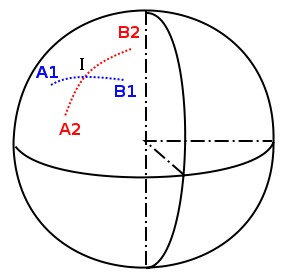
\includegraphics[width=5cm]{images/Sphere.png}
    \caption{Représentation grossière de l'interssection de deux arc de cercle respectivement formé par la trajectoire la plus courte entre deux points situé sur le Globe terrestre}
    \label{sphere}
\end{figure}
            \paragraph{Résolution:}
Étant donné que j'ai effectué un BTS avant d'intégrer l'EIGSI \footnote{EIGSI: École d'Ingénieurs en Génie des Systèmes Industriel située à La Rochelle}, les notion de coordonnées sphérique ne me sont que peut familière. Après avoir en vainc cherché sur internet ainsi que dans mon entourage  (maître de stage, collègues de travail) je me suis replié sur un forum de mathématique sur le quel j'ai déposé un sujet explicitant le problème (adresse, cf. bibliographie \cite{forummath}). Une personne nous a donnée une solution qui, après connaissance, semble tellement simple qu'on se demande pourquoi personne n'y a pensés. Cette solution consiste a déterminer les plan défini par les deux points aux extremités de chaques arc et par le centre de la terre (ainsi nous avons forcement la courbe qu'a suivi l'avion sur ce plan). Il faut ensuite déterminer la normal a chacun des plan pour en déduire la droite d'intersection de ces plan (passant par le centre de la sphère). Une foi cette droite acquise il faut définir sont vecteur norme et le convertir en coordonnée sphérique. Ce qui nous donne un des point d'intersection de la droite avec la sphère, l'autre étant situé par définition à l'opposé.

Une démonstration valant amplement un long discours, et a titre informatif, voici ce que cela donne en résolution mathématique. Pour cet exemple nous avons deux arcs représentent 2 trajectoires difinie chaqune par 2 points A et B (cf. Fig. \vref{sphere}). Chaque pour sera defini par une latitude et une longitude.

\begin{itemize}
    \item Nous avons donc:
    \begin{itemize}
        \item $lat_{A}$ la latitude de A
        \item $long_{A}$ la longitude de A
        \item $(x_{A}, y_{A}, z_{A})$ les coordonées cartésiennes de A
        \item $I_{1}$ le point d'intersection \no 1
        \item $I_{2}$ le point d'intersection \no 2
    \end{itemize}
    \item Il faut tout d'abord convertir les coordonnées sphérique en vecteur de coordonnées cartésiennes pour $A$ et $B$:
    $$  A=\left\{
    \begin{array}{rcl}x_A & = & cos(lat) \times cos(long)\\ y_D & = & cos(lat_{A}) \times sin(long_{A})\\ z_A & = & sin(lat_{A}) 
    \end{array}\right.$$
    \item Il faut ensuite déterminer le plan passant par $O$, $A$ et $B$ ayant alors pour équation:
    $$ax+by+cz=0$$ où $$\left(\matrix {a\cr b\cr c}\right)= \left(\matrix {x_A\cr y_A\cr z_A}\right)\wedge \left(\matrix {x_B\cr y_B\cr z_B}\right)$$c'est à dire $$\left\{\matrix {a=y_Az_B-z_Ay_B\cr b=z_Ax_B-x_Az_B\cr c=x_Ay_B-y_Ax_B}\right.$$
    \item L'intersection des deux plans de coordonées $(a,b,c)$ et (a',b',c') contient le point O, mais aussi le point $P$ de coordonnées $(x_P,y_P,z_P)$ tel que: $$\left(\matrix {x_P\cr y_P\cr z_P}\right)= \left(\matrix {a\cr b\cr c}\right)\wedge \left(\matrix {a'\cr b'\cr c'}\right)$$
    \item P n'ettant pas forcément sur la sphère, il faut trouver un point de la droite $(OP)$ sur cette sphère. Pour cela il suffit de diviser les 3 coordonnées de P par la norme de $\overrightarrow{OP}$:
    $$I_{1} = \left\{\matrix {x_P / \sqrt{x_P^2+y_P^2+z_P^2}\cr x_P / \sqrt{y_P^2+y_P^2+z_P^2}\cr x_P / \sqrt{z_P^2+y_P^2+z_P^2}}\right.$$
    \item nous avons donc $I_1$ et son opposé $I_2$, il nous reste donc plus qu'a verifier si chaqun de ces points appartient à un des 2 arcs.
\end{itemize}
Vous trouverez le code Python correspondant à ces calcule dans la fonction: "verifyIntersection (line, point):" du module "ususalFonction.py" disponible en annexe \vref{usualfonction}

    \subsection{Performance du logiciel\label{perf}}
            \paragraph{Problématique:}
Les premiers tests du logiciel ce sont déroulé sur un nombre limité de fichiers (représenté par un nombre limité d'heure de vol), ce affin de pouvoir les valider rapidement. Lors de l'apparition de fichiers plus volumineux (plus de 300Mo de donnée en entrée, environ 10\% en sortie) c'est posé le probleme de performancee. Avant optimisation l'ordinateur moulinais des heures avant de pouvoir sortir un fichier. Il a donc falut optimiser le code afin d'alleger le programe en resources.

            \paragraph{Résolution:}
En cherchant des conseils dans des forum d'informatique ainsi que dans le livre cité précédement (cf. bibliographie \cite{pybook}, nous avons découvert que Python etait un langage orientier par les test et qu'il disposait donc de librairies spécialment conçues pour determiner les point bloquant d'un programme et les foctions appelées les plus gourmandes.

La fonction retenue pour repérer ce qui est appelé en anglais les Bottleneck\footnote{Bottlneck: (goulot d'étranglement) point d'un système limitant les performances globales, et pouvant avoir un effet sur les temps de traitement et de réponse.} est la fonction "hotshot" qui à pour but d'analyser un programme dans sa totalité en indiquant nottament les resources utilisées par chaque fonction appelée. Pour visualiser ce que donne le résultat d'une analyse veuillez vous reporter a la figure \vref{stat}.

Les bottlenecks reperés, une réecriture des parties bloquantes à du être effectuée. Cette analyse nous a permis de réduire les ressources et donc le temps d'execution du logiciel de plus de 80\%.
